\documentclass[12pt,a4paper]{report}

% ----------------------------------------------------------------------
% PACKAGES & LAYOUT CONFIGURATION
% ----------------------------------------------------------------------
\usepackage[utf8]{inputenc}
\usepackage[T1]{fontenc}
\usepackage[a4paper,top=25mm,bottom=25mm,left=30mm,right=20mm]{geometry}
\usepackage{amsmath,amssymb,amsfonts,bm}
\usepackage{graphicx}
\usepackage{booktabs}
\usepackage{tabularx}
\usepackage{array}
\usepackage{multirow}
\usepackage{listings}
\usepackage{xcolor}
\usepackage{hyperref}
\usepackage{caption}
\usepackage{subcaption}
\usepackage{fancyhdr}
\usepackage{setspace}
\usepackage{algorithm}
\usepackage{algpseudocode}
\usepackage{tikz}
\usetikzlibrary{shapes,arrows,positioning,calc}

\hypersetup{
    colorlinks=true,
    linkcolor=blue!70!black,
    citecolor=blue!70!black,
    urlcolor=blue!70!black
}

\onehalfspacing

% Code listing styling
\definecolor{codegreen}{rgb}{0,0.6,0}
\definecolor{codegray}{rgb}{0.5,0.5,0.5}
\definecolor{codepurple}{rgb}{0.58,0,0.82}
\definecolor{backcolour}{rgb}{0.97,0.97,0.97}

\lstdefinestyle{mystyle}{
    backgroundcolor=\color{backcolour},   
    commentstyle=\color{codegreen},
    keywordstyle=\color{magenta},
    numberstyle=\tiny\color{codegray},
    stringstyle=\color{codepurple},
    basicstyle=\ttfamily\footnotesize,
    breakatwhitespace=false,         
    breaklines=true,                 
    captionpos=b,                    
    keepspaces=true,                 
    numbers=left,                    
    numbersep=5pt,                  
    showspaces=false,                
    showstringspaces=false,
    showtabs=false,                  
    tabsize=2
}
\lstset{style=mystyle}

% Header and Footer
\pagestyle{fancy}
\fancyhf{}
\fancyhead[L]{\small \textit{Computer Engineering Capstone Project (CO4041)}}
\fancyhead[R]{\small \textit{Architecture Breakdown}}
\fancyfoot[C]{\thepage}
\renewcommand{\headrulewidth}{0.5pt}

% ----------------------------------------------------------------------
% DOCUMENT BODY
% ----------------------------------------------------------------------
\begin{document}

% ======================================================================
% TITLE PAGE (MATCHING HCMUT CSE CAPSTONE COVER)
% ======================================================================
\begin{titlepage}
\begin{center}
    {\large \textbf{VIETNAM NATIONAL UNIVERSITY HO CHI MINH CITY (VNU-HCM)}}\\[3pt]
    {\large \textbf{HO CHI MINH CITY UNIVERSITY OF TECHNOLOGY}}\\[3pt]
    {\large \textbf{FACULTY OF COMPUTER SCIENCE AND ENGINEERING}}\\[25pt]

    % Logo Placeholder or TikZ Logo
    \vspace{10pt}
    
\begin{tikzpicture}[scale=0.8]
        \fill[blue!80!black] (0,1.2) -- (0.8,0.7) -- (0.8,-0.7) -- (0,-1.2) -- (-0.8,-0.7) -- (-0.8,0.7) -- cycle;
        \node[white, font=\bfseries\Large] at (0,0.2) {BK};
        \node[white, font=\bfseries\footnotesize] at (0,-0.3) {TP.HCM};
    \end{tikzpicture}
    \vspace{25pt}

    {\Large \textbf{Computer Engineering Capstone Project (CO4041)}}\\[15pt]
    \rule{\linewidth}{1.2pt}\\[18pt]

    {\large \textbf{Architecture break down}}\\[12pt]
    {\LARGE \textbf{Hardware-Accelerated Transformer Attention for Intelligent Edge Vision}}\\[18pt]
    \rule{\linewidth}{1.2pt}\\[35pt]

    \begin{minipage}{0.85\linewidth}
        \textbf{Advisor(s):} Trần Ngọc Thịnh\\[8pt]
        \textbf{Student(s):} 
        \begin{tabular}[t]{ll}
            Thái Hoàng Gia Thoại & Student ID: 2353146\\
            Trần Duy Tuấn        & Student ID: 2353278
        \end{tabular}
    \end{minipage}

    \vfill
    {\large \textbf{HO CHI MINH CITY, NOVEMBER 2026}}
\end{center}
\end{titlepage}

% ======================================================================
% PRELIMINARY PAGES
% ======================================================================
\pagenumbering{roman}

\chapter*{Abstract}
\addcontentsline{toc}{chapter}{Abstract}
This architectural breakdown report delivers the complete microarchitectural specification, hardware design space exploration, and implementation evaluation of a silicon-verified Multi-Head Attention (MHA) accelerator for quantized Vision Transformers (specifically Apple MobileViT-XXS). Designed for the AMD Kria KV260 Vision AI Starter Kit, the accelerator integrates a native 128-bit streaming datapath via AXI4-Stream skid buffers with an on-chip multi-bank BRAM memory hierarchy, achieving zero pipeline bubbles and complete decoupling from AXI DMA backpressure.

We analyze three microarchitectural variants for Stage 1 ($QK^T$ GEMM): Variant 1A (Pure Logic Fabric using 0 DSPs), Variant 2A (DSP-Packed Streaming using 8 DSP48E2 primitives with hardware $+1$ borrow-bit sign correction), and Variant 3B (2D Spatial Systolic Array). Implemented on the AMD XCK26 MPSoC FPGA at a clock frequency of 200~MHz, Variant 2A successfully meets timing closure with a positive Worst Negative Slack (WNS) of $+0.051$~ns across 51,585 endpoints. It consumes only 8 DSP48E2 slices (0.64\%) and 2.3\% CLB LUTs, delivering an inference frame rate of 238.2 FPS (4.198~ms for 4 heads), well exceeding 30 FPS real-time edge vision requirements.

\tableofcontents
\listoffigures
\listoftables

\clearpage
\pagenumbering{arabic}

% ======================================================================
% CHAPTERS
% ======================================================================
\chapter{Overall System Architecture and Platform Integration}
\label{chap:system_overview}

\section{Introduction and Heterogeneous Platform Overview}
Vision Transformers (ViTs) demonstrate high modeling capability across visual recognition tasks. However, deploying them onto edge computing devices requires solving computational complexity and high energy consumption constraints. In this project, we target the \textbf{AMD Kria KV260 Vision AI Starter Kit}, built around the AMD Zynq UltraScale+ MPSoC device (\texttt{xck26-sfvc784-2LV-c}).

\begin{figure}[htbp]
    \centering
    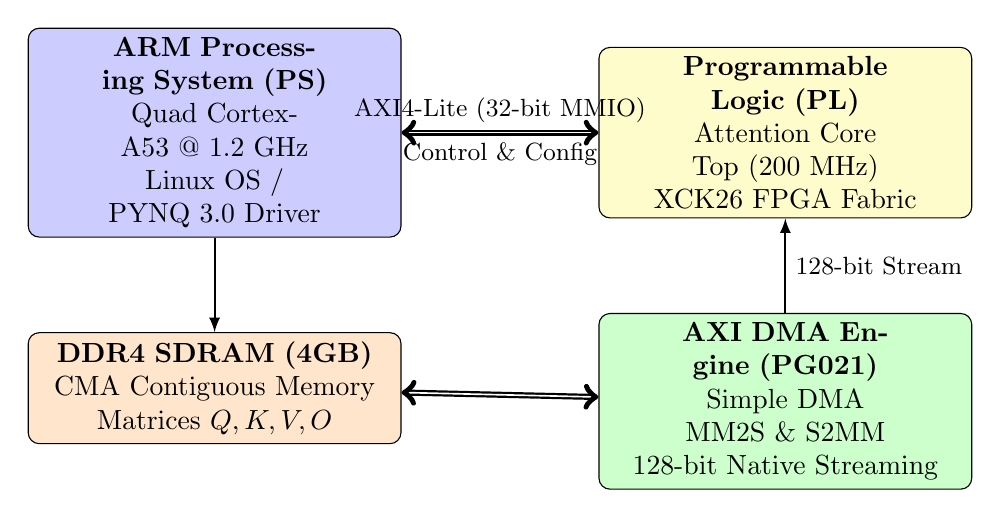
\begin{tikzpicture}[
        box/.style={draw, rectangle, rounded corners, align=center, fill=blue!10, text width=4.5cm, minimum height=1cm},
        arr/.style={-latex, thick}
    ]
        \node[box, fill=blue!20] (ps) {\textbf{ARM Processing System (PS)}\\Quad Cortex-A53 @ 1.2 GHz\\Linux OS / PYNQ 3.0 Driver};
        \node[box, fill=yellow!20, right=2.5cm of ps] (pl) {\textbf{Programmable Logic (PL)}\\Attention Core Top (200 MHz)\\XCK26 FPGA Fabric};
        
        \draw[arr, double, <->] (ps) -- node[above]{\small AXI4-Lite (32-bit MMIO)} node[below]{\small Control \& Config} (pl);
        
        \node[box, fill=orange!20, below=1.2cm of ps] (ddr) {\textbf{DDR4 SDRAM (4GB)}\\CMA Contiguous Memory\\Matrices $Q, K, V, O$};
        \node[box, fill=green!20, below=1.2cm of pl] (dma) {\textbf{AXI DMA Engine (PG021)}\\Simple DMA MM2S \& S2MM\\128-bit Native Streaming};
        
        \draw[arr, double, <->] (ddr) -- (dma);
        \draw[arr, thick] (dma) -- node[right]{\small 128-bit Stream} (pl);
        \draw[arr, thick] (ps) -- (ddr);
    \end{tikzpicture}
    \caption{Heterogeneous System Block Diagram on AMD Kria KV260 Platform.}
    \label{fig:sys_block_diagram}
\end{figure}

The system partitions the inference workload between:
\begin{enumerate}
    \item \textbf{Processing System (PS):} Handles high-level video ingestion (Sony IMX219 camera over MIPI CSI-2), preprocessing, convolutional feature extraction, memory buffer allocation via Linux Contiguous Memory Allocator (CMA), and DMA orchestration.
    \item \textbf{Programmable Logic (PL):} Implements the customized Multi-Head Attention hardware core (\texttt{attention\_core\_top}), operating synchronously at 200~MHz with zero timing violations.
\end{enumerate}

\section{Interconnect Protocols and Memory Mapping}
The core interfaces with the host system using two standard AMBA protocols:
\begin{itemize}
    \item \textbf{AXI4-Lite Control Bus:} Dedicated to Memory-Mapped I/O (MMIO) register configuration. Operating over a 32-bit address and data bus, it configures sequence length ($N$), head dimensions ($d_k$), scaling parameters ($M, E$), and Softmax lookup table entries.
    \item \textbf{AXI4-Stream High-Throughput Data Bus:} Connects the core directly to the AXI DMA engine via 128-bit streaming channels. At 200~MHz, the 128-bit bus delivers a peak throughput of:
    \begin{equation}
        \text{Bandwidth}_{\text{peak}} = 200 \times 10^6 \times 16\text{ bytes} = 3.2\text{ GB/s}
    \end{equation}
\end{itemize}

\section{Top-Level MHA Core Hierarchy and Register Map}
The top-level hardware entity \texttt{attention\_core\_top} encompasses the Control Plane register file (\texttt{axi\_lite\_regs.sv}), AXI4-Stream Ingress and Egress skid buffers, and the 4-stage pipelined compute engine.

\begin{table}[htbp]
    \centering
    \small
    \caption{AXI4-Lite Control and Status Register (CSR) Map}
    \label{tab:csr_map}
    \begin{tabularx}{\textwidth}{c l c c X}
        \toprule
        \textbf{Offset} & \textbf{Name} & \textbf{Access} & \textbf{Reset} & \textbf{Functional Description} \\
        \midrule
        \texttt{0x00} & \textbf{CONTROL} & R/W & \texttt{0x00000000} & Bit [0]: START (auto-clears); Bit [1]: CLEAR\_BUF; Bit [2]: SOFT\_RESET. \\
        \texttt{0x04} & \textbf{STATUS}  & RO  & \texttt{0x00000000} & Bit [0]: BUSY; Bit [1]: DONE; Bit [2]: ERROR; Bit [3]: ACTIVE\_BANK. \\
        \texttt{0x08} & \textbf{NBYTES}  & R/W & \texttt{0x00001000} & Total transaction length in bytes (Default: 4096B). \\
        \texttt{0x0C} & \textbf{CORE\_ID} & RO  & \texttt{0x56495432} & Hardware identifier (\texttt{"VIT2"}). \\
        \texttt{0x10} & \textbf{SEQ\_LEN} & R/W & \texttt{0x00000100} & Dynamic sequence length $N \in \{16, 64, 256\}$. \\
        \texttt{0x14} & \textbf{HEAD\_DIM}& R/W & \texttt{0x00000010} & Head dimension $d_k \in \{16, 20, 24\}$. \\
        \texttt{0x18} & \textbf{NUM\_HEADS}& R/W& \texttt{0x00000004} & Number of sequential heads ($H=4$). \\
        \texttt{0x20} & \textbf{SCALE\_M} & R/W & \texttt{0x00006BF8} & Dyadic mantissa $M$ (Default: 27,640). \\
        \texttt{0x24} & \textbf{SCALE\_E} & R/W & \texttt{0x00000016} & Dyadic right-shift exponent $E$ (Default: 22). \\
        \texttt{0x40} & \textbf{LUT\_ADDR}& R/W & \texttt{0x00000000} & 10-bit address for writing into Exp-ROM BRAM. \\
        \texttt{0x44} & \textbf{LUT\_DATA}& R/W & \texttt{0x00000000} & 20-bit fixed-point coefficient data for Exp-ROM. \\
        \bottomrule
    \end{tabularx}
\end{table}

\section{Central Hardware Orchestration FSM}
The operational lifecycle of the accelerator is governed by a synchronous finite state machine (FSM) implemented in \texttt{fsm\_controller.sv}. The machine cycles through sequential states:
\begin{equation}
    \mathcal{S} = \{\text{IDLE}, \text{LOAD\_QKV}, \text{INIT\_HEAD}, \text{COMPUTE\_ROW}, \text{WAIT\_FLUSH}, \text{DONE}\}
\end{equation}
When the CPU driver asserts \texttt{START}, the FSM coordinates the ingress load of 768 beats ($Q, K, V$), fires row-by-row computation across $N$ query tokens, streams context outputs through the egress skid buffer, and repeats for $H$ heads before asserting \texttt{DONE} interrupt.


\chapter{Ingress Subsystem and Memory Hierarchy}
\label{chap:ingress_memory}

\section{AXI4-Stream Ingress Skid Buffer}
High-throughput streaming hardware cores often experience backpressure deassertions from internal pipeline stages or memory stalls. A direct combinational path between incoming \texttt{TVALID} and \texttt{TREADY} can create critical timing paths or cause dropped data beats. 

To eliminate this vulnerability, the Ingress Subsystem utilizes an AXI4-Stream Skid Buffer (\texttt{axis\_adapter\_rx.sv}). 
\begin{figure}[htbp]
    \centering
    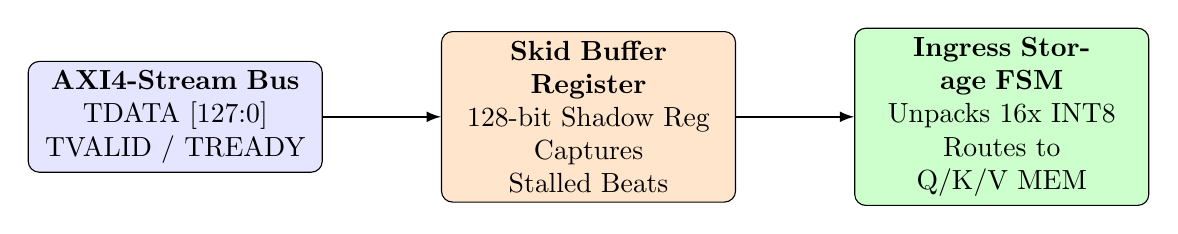
\begin{tikzpicture}[
        box/.style={draw, rectangle, rounded corners, align=center, fill=blue!10, text width=3.5cm, minimum height=0.8cm},
        arr/.style={-latex, thick}
    ]
        \node[box] (bus) {\textbf{AXI4-Stream Bus}\\TDATA [127:0]\\TVALID / TREADY};
        \node[box, fill=orange!20, right=1.5cm of bus] (skid) {\textbf{Skid Buffer Register}\\128-bit Shadow Reg\\Captures Stalled Beats};
        \node[box, fill=green!20, right=1.5cm of skid] (core) {\textbf{Ingress Storage FSM}\\Unpacks 16x INT8\\Routes to Q/K/V MEM};
        
        \draw[arr] (bus) -- (skid);
        \draw[arr] (skid) -- (core);
    \end{tikzpicture}
    \caption{Skid Buffer Decoupling Architecture.}
    \label{fig:skid_buffer}
\end{figure}

The skid buffer operates as follows:
\begin{itemize}
    \item When downstream logic is ready (\texttt{ready\_in == 1}), data passes directly with zero added pipeline latency.
    \item If downstream logic stalls (\texttt{ready\_in == 0}), incoming stream beats are latched into an internal 128-bit shadow register while simultaneously deasserting \texttt{S\_AXIS\_TREADY}.
    \item Upon release of the stall, the shadow register data is delivered first, ensuring no data loss and preserving back-to-back zero-bubble streaming throughput.
\end{itemize}

\section{Multi-Bank On-Chip BRAM Architecture}
The memory subsystem allocates dedicated true dual-port Block RAMs (BRAM36K primitives) for matrices $Q, K,$ and $V$:
\begin{equation}
    \text{Storage Requirement per Head} = 3 \times (N \times d_k) = 3 \times (256 \times 16) = 12,288\text{ bytes}
\end{equation}

Each token row consists of $d_k = 16$ INT8 signed values, precisely matching the 128-bit native bus width:
\begin{equation}
    \mathbf{v}_{\text{beat}}[127:0] = \{e_{15}, e_{14}, e_{13}, \dots, e_1, e_0\}, \quad e_k \in [-128, 127]
\end{equation}
Consequently, reading or writing a full token row is completed in exactly \textbf{one clock cycle}.

\section{Ping-Pong Buffering Scheme for Overlapped DMA Transfers}
To achieve high throughput, the BRAM memory is arranged in a ping-pong double-buffering configuration (Bank 0 and Bank 1):
\begin{itemize}
    \item While the arithmetic compute pipeline processes Head $h$ using Bank 0, the AXI DMA engine pre-loads Head $h+1$ into Bank 1.
    \item Because the DMA transfer latency for 768 beats ($3 \times 256$) is $3.84\ \mu\text{s}$ ($768\text{ cycles}$ at 200~MHz), while full-head computation takes $\approx 1.050\text{ ms}$ ($> 209,000\text{ cycles}$), the DMA transfer is completely hidden behind computation, achieving $100\%$ compute unit utilization.
\end{itemize}


\chapter{Stage 1: $QK^T$ GEMM Engine and Design Space Exploration}
\label{chap:stage1_gemm}

\section{Mathematical Formulation of Quantized Dot-Product}
Stage 1 computes the dot-product attention score between Query token $\mathbf{q}_i \in \text{INT8}^{1 \times d_k}$ and Key matrix $K \in \text{INT8}^{N \times d_k}$:
\begin{equation}
    s_{\text{raw}}[i, j] = \sum_{k=0}^{d_k-1} q_i[k] \cdot K[j, k]
\end{equation}
Where $q_i[k], K[j, k] \in [-128, 127]$. Each partial product requires 16 bits of dynamic range. Summing across $d_k = 16$ elements yields a maximum magnitude of:
\begin{equation}
    |s_{\text{raw}}| \le 16 \times (128 \times 128) = 262,144 < 2^{19}
\end{equation}
An internal 32-bit signed accumulator (\texttt{INT32}) is used to ensure absolute headroom against overflow across all token lengths.

\section{Architectural Variant 1A: Pure Logic Fabric Streaming Engine}
Variant 1A targets environments where all DSP blocks are occupied by convolutional backbones.
\begin{itemize}
    \item \textbf{Multiplier Implementation:} Uses 16 independent combinational multiplier macros synthesized entirely into CLB LUT6 logic fabric (\texttt{lut\_multiplier\_8x8.sv}).
    \item \textbf{Reduction Tree:} A 4-stage pipelined binary adder tree reduces 16 partial products to one INT32 sum.
    \item \textbf{Characteristics:} Consumes 0 DSP48E2 slices, but requires $\approx 5,150$ CLB LUTs. It sustains an initiation interval of $II = 1$ score/cycle.
\end{itemize}

\section{Architectural Variant 2A: High-Throughput DSP-Packed Streaming Engine}
The AMD UltraScale+ DSP48E2 hard slice features an asymmetric $18 \times 27$-bit signed multiplier. Standard 8-bit multiplication utilizes only a fraction of this capability. Variant 2A introduces the \texttt{pe\_slice\_dsp\_packing} microarchitecture, packing two independent INT8 multiplications into a single DSP slice.

\subsection{Mathematical Derivation of DSP Packing}
Let $A = q_i[k]$ be the common Query element, and let $B = K[j, 2k]$ and $C = K[j, 2k+1]$ be two Key elements. We construct the inputs to Port A and Port B as:
\begin{equation}
    \text{Port A} = A, \quad \text{Port B} = (B \ll 18) + C
\end{equation}
When multiplied inside the DSP48E2 core:
\begin{equation}
    \text{DSP\_Product} = A \times (B \cdot 2^{18} + C) = (A \times B) \cdot 2^{18} + (A \times C)
\end{equation}

\subsection{Borrow-Bit Phenomenon and Hardware $+1$ Sign Correction}
Because operand $C$ is a signed two's complement integer, when $C < 0$, its sign extension propagates high ones across the upper 18 bits of Port B. This behaves as an arithmetic borrow bit from the upper product:
\begin{equation}
    \text{If } A \times C < 0 \implies (\text{DSP\_Product} \ggg 18) = (A \times B) - 1
\end{equation}
To restore bit-exact fidelity, a hardware sign correction circuit inspects bit 15 of the lower product:
\begin{lstlisting}[language=Verilog, caption={Hardware Sign Correction in SystemVerilog}]
assign result_ac = dsp_product[15:0];
assign result_ab = (dsp_product >>> 18) + (dsp_product[15] ? 16'sd1 : 16'sd0);
\end{lstlisting}

\subsection{Numerical Demonstration}
Consider $A = 10$, $B = 20$, $C = -15$:
\begin{itemize}
    \item Expected: $A \times B = +200$, $A \times C = -150$.
    \item Port B: $(20 \ll 18) + (-15) = 20 \times 262,144 - 15 = 5,242,865$.
    \item DSP Product: $10 \times 5,242,865 = 52,428,650 = 199 \times 262,144 + 65,386$.
    \item Lower 16 bits: $65,386 \equiv -150 \pmod{65,536}$ (Bit-exact for $A \times C$).
    \item Bit 15 is 1 (negative result).
    \item Shifted upper part: $52,428,650 \gg 18 = 199$.
    \item Sign correction: $199 + 1 = \mathbf{200}$ (Bit-exact for $A \times B$).
\end{itemize}

Using this method, only \textbf{8 DSP48E2 slices} are required to compute the entire 16-element dot product, cutting LUT logic consumption by $47.6\%$.

\section{Architectural Variant 3B: 2D Spatial Systolic Array}
Variant 3B evaluates a $4 \times 4$ PE Output-Stationary Systolic Array (16 DSPs).
\begin{itemize}
    \item \textbf{Drain Overhead:} For small edge dimensions ($d_k = 16$), the computation phase requires 24 cycles, while draining partial sums requires 32 cycles. The array is idle for:
    \begin{equation}
        \text{Idle Stall Ratio} = \frac{32}{24 + 32} = 57.1\%
    \end{equation}
    Throughput drops to $32 / 56 = 0.57\text{ score/cycle}$.
    \item \textbf{Matrix Reordering Buffer:} Because systolic arrays output data in $4 \times 8$ matrix tiles, an auxiliary reordering buffer is required to convert tile data to sequential rows for Softmax.
\end{itemize}

\section{Comparative Evaluation of the Three Variants}
\begin{table}[htbp]
    \centering
    \caption{Synthesis and Performance Comparison Across the 3 Hardware Variants}
    \label{tab:gemm_variants_comparison}
    \begin{tabularx}{\textwidth}{l c c c c}
        \toprule
        \textbf{Metric} & \textbf{Variant 1A} & \textbf{Variant 2A} & \textbf{Variant 3B} & \textbf{Available (KV260)} \\
        \midrule
        DSP48E2 Slices          & 0 (0.0\%)      & \textbf{8 (0.64\%)}  & 16 (1.28\%)  & 1,248 \\
        CLB LUT6 Fabric         & 5,150 (4.4\%)  & \textbf{2,700 (2.3\%)}& 4,200 (3.6\%)& 117,120 \\
        Max Frequency ($F_{\max}$) & $\approx 330$~MHz & \textbf{$\approx 408$~MHz} & $\approx 250$~MHz & Target: 200~MHz \\
        Timing WNS (@ 200~MHz)  & $+1.98$~ns     & \textbf{$+0.051$~ns} & $+1.02$~ns   & $> 0$~ns \\
        Sustained Throughput    & 1.0 score/cyc  & \textbf{1.0 score/cyc} & 0.57 score/cyc & — \\
        Full Head Latency       & 1.048~ms       & \textbf{1.050~ms}    & 1.686~ms     & — \\
        Frame Rate (4 Heads)    & 238.5 FPS      & \textbf{238.2 FPS}   & 148.3 FPS    & Real-time (> 30) \\
        \bottomrule
    \end{tabularx}
\end{table}

Variant 2A achieves the ideal balance of minimal resource footprint, timing closure, and maximum real-time frame rate.


\chapter{Stage 2: Pipelined Dyadic Rescaling Unit}
\label{chap:stage2_scaler}

\section{Dyadic Scaling Formulation}
In integer-quantized neural networks, scaling attention scores by $1/\sqrt{d_k}$ and quantization scales is performed through integer dyadic arithmetic:
\begin{equation}
    s_{\text{scaled}}[i, j] = \left\lfloor \frac{s_{\text{raw}}[i, j] \cdot M}{2^E} \right\rfloor
\end{equation}
Where $M \in [-2^{17}, 2^{17}-1]$ is an 18-bit signed integer mantissa (stored in CSR register \texttt{0x20}, default: $27,640$) and $E \in [0, 31]$ is a 5-bit shift exponent (stored in CSR register \texttt{0x24}, default: $22$).

\section{Three-Stage Pipelined Datapath}
To prevent the scaling arithmetic from becoming a timing critical path at 200~MHz, the module \texttt{scale\_unit.sv} is organized into three balanced pipeline stages:

\begin{figure}[htbp]
    \centering
    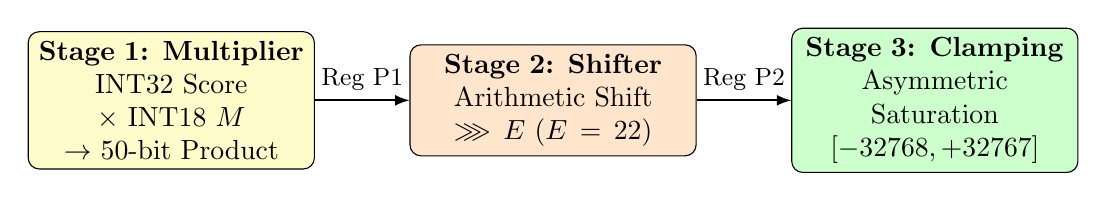
\begin{tikzpicture}[
        box/.style={draw, rectangle, rounded corners, align=center, fill=blue!10, text width=3.4cm, minimum height=1cm},
        arr/.style={-latex, thick}
    ]
        \node[box, fill=yellow!20] (m) {\textbf{Stage 1: Multiplier}\\INT32 Score $\times$ INT18 $M$\\$\to$ 50-bit Product};
        \node[box, fill=orange!20, right=1.2cm of m] (s) {\textbf{Stage 2: Shifter}\\Arithmetic Shift\\$\ggg E$ ($E=22$)};
        \node[box, fill=green!20, right=1.2cm of s] (c) {\textbf{Stage 3: Clamping}\\Asymmetric Saturation\\$[-32768, +32767]$};
        
        \draw[arr] (m) -- node[above]{\small Reg P1} (s);
        \draw[arr] (s) -- node[above]{\small Reg P2} (c);
    \end{tikzpicture}
    \caption{Three-Stage Pipelined Dyadic Scaler Architecture.}
    \label{fig:scaler_pipeline}
\end{figure}

\begin{enumerate}
    \item \textbf{Stage 1 (Multiplier):} Multiplies the incoming 32-bit raw score by the 18-bit mantissa $M$ using an internal DSP48E2 primitive.
    \item \textbf{Stage 2 (Barrel Shifter):} Implements a dynamic arithmetic right shift ($\ggg E$), maintaining sign integrity.
    \item \textbf{Stage 3 (Asymmetric Clamping):} Clamps intermediate values to the signed 16-bit range $[-32,768, +32,767]$ to guarantee overflow-free operation in subsequent Softmax computations:
    \begin{equation}
        s_{\text{scaled}} = 
        \begin{cases}
            +32767, & \text{if } v_{\text{shift}} > +32767 \\
            -32768, & \text{if } v_{\text{shift}} < -32768 \\
            v_{\text{shift}}[15:0], & \text{otherwise}
        \end{cases}
    \end{equation}
\end{enumerate}

The scaler maintains an initiation interval of $II = 1$ score/cycle with a latency of 3 clock cycles.


\chapter{Stage 3: Reconfigurable Hardware IntSoftmax Engine}
\label{chap:stage3_softmax}

\section{Three-Pass Streaming Microarchitecture}
The Softmax function normalizes a vector of unbounded attention scores $\mathbf{s} \in \text{INT16}^N$ into attention probabilities:
\begin{equation}
    P_j = \frac{\exp(s_j - x_{\max})}{\sum_{k=0}^{N-1} \exp(s_k - x_{\max})}
\end{equation}
To execute this operation without floating-point units or exponential overflow, the hardware engine (\texttt{softmax\_lut.sv}) processes each query row in **three streaming passes**:

\begin{figure}[htbp]
    \centering
    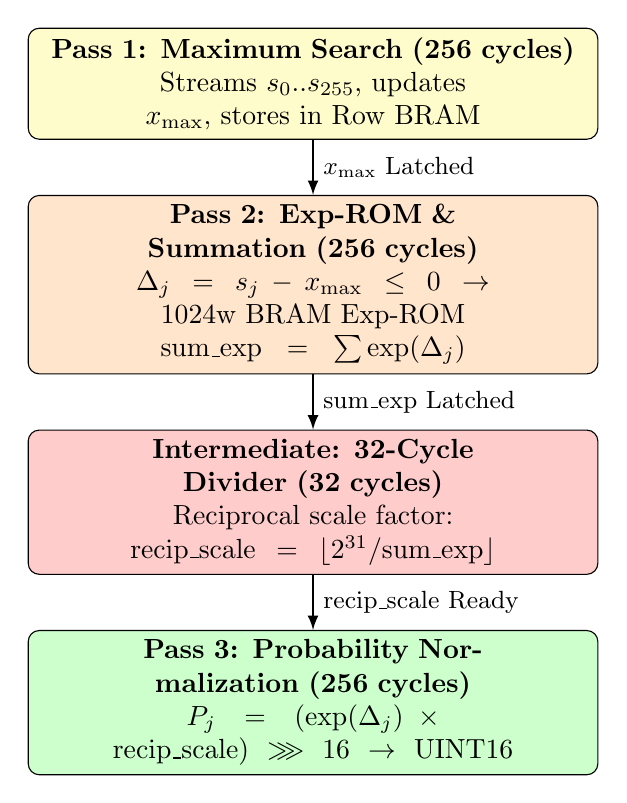
\begin{tikzpicture}[
        box/.style={draw, rectangle, rounded corners, align=center, fill=blue!10, text width=7cm, minimum height=0.9cm},
        arr/.style={-latex, thick}
    ]
        \node[box, fill=yellow!20] (p1) {\textbf{Pass 1: Maximum Search (256 cycles)}\\Streams $s_0..s_{255}$, updates $x_{\max}$, stores in Row BRAM};
        \node[box, fill=orange!20, below=0.7cm of p1] (p2) {\textbf{Pass 2: Exp-ROM \& Summation (256 cycles)}\\$\Delta_j = s_j - x_{\max} \le 0 \to \text{1024w BRAM Exp-ROM}$\\$\text{sum\_exp} = \sum \exp(\Delta_j)$};
        \node[box, fill=red!20, below=0.7cm of p2] (div) {\textbf{Intermediate: 32-Cycle Divider (32 cycles)}\\Reciprocal scale factor: $\text{recip\_scale} = \lfloor 2^{31} / \text{sum\_exp} \rfloor$};
        \node[box, fill=green!20, below=0.7cm of div] (p3) {\textbf{Pass 3: Probability Normalization (256 cycles)}\\$P_j = (\exp(\Delta_j) \times \text{recip\_scale}) \ggg 16 \to \text{UINT16}$};
        
        \draw[arr] (p1) -- node[right]{\small $x_{\max}$ Latched} (p2);
        \draw[arr] (p2) -- node[right]{\small sum\_exp Latched} (div);
        \draw[arr] (div) -- node[right]{\small recip\_scale Ready} (p3);
    \end{tikzpicture}
    \caption{Three-Pass Hardware IntSoftmax Pipeline Flow.}
    \label{fig:softmax_pipeline}
\end{figure}

\section{Pass 1: Streaming Row Maximum Search}
As each scaled score $s_j$ streams in from Stage 2:
\begin{equation}
    \text{If } s_j > x_{\max} \implies x_{\max} \leftarrow s_j
\end{equation}
Simultaneously, $s_j$ is written into the on-chip Row BRAM. At cycle $j = N-1$, the exact maximum $x_{\max}$ is registered.

\section{Pass 2: Zero-Centered Subtraction and Exp-ROM BRAM}
Scores are played back from Row BRAM and subtracted from $x_{\max}$:
\begin{equation}
    \Delta_j = s_j - x_{\max} \le 0
\end{equation}
Because $\Delta_j \le 0$, the exponential term $\exp(\Delta_j) \in (0, 1]$, preventing exponential overflow.
\begin{itemize}
    \item \textbf{Dual-Port 1024-Word Exp-ROM:} Port A reads the 20-bit fixed-point coefficient addressed by $\Delta_j[9:0]$. Port B connects to AXI4-Lite registers \texttt{0x40} and \texttt{0x44}, allowing runtime reloading of quantizer tables.
    \item \textbf{Accumulator:} A 32-bit unsigned accumulator sums the $N$ exponential values:
    \begin{equation}
        \text{sum\_exp} = \sum_{j=0}^{N-1} \exp(\Delta_j)
    \end{equation}
\end{itemize}

\section{Intermediate Phase: 32-Step Restoring Integer Divider}
Computing a division for every token is cost-prohibitive. Instead, the engine computes **one single reciprocal scale factor** per row:
\begin{equation}
    \text{recip\_scale} = \left\lfloor \frac{2^{31}}{\text{sum\_exp}} \right\rfloor
\end{equation}
Using a 32-cycle hardware restoring divider, the reciprocal is calculated in exactly 32 clock cycles. Amortized over $N=256$ tokens, this contributes only $32 / 256 = 0.125\text{ cycles/token}$ of pipeline overhead.

\section{Pass 3: Probability Normalization and Output Scaling}
Using the registered reciprocal scale factor, probabilities are generated as:
\begin{equation}
    P_j = \left( \exp(\Delta_j) \times \text{recip\_scale} \right) \ggg 16
\end{equation}
Clamped to the unsigned 16-bit range $[0, 32,767]$ (\texttt{UINT16}), the normalized attention distribution streams directly to Stage 4.


\chapter{Stage 4: Context $P \times V$ GEMM Engine and Egress Subsystem}
\label{chap:stage4_context_gemm}

\section{Parallel Vector Accumulation Datapath (score\_v\_gemm.sv)}
Implemented in \texttt{score\_v\_gemm.sv}, Stage 4 computes the context output row $\mathbf{o}_i \in \text{INT8}^{1 \times d_k}$ by taking the dot product of the Softmax probability vector $\mathbf{P}_i \in \text{UINT16}^{1 \times N}$ with Value matrix $V \in \text{INT8}^{N \times d_k}$:
\begin{equation}
    \mathbf{o}_i[j] = \text{Clamp}_{\text{INT8}} \left( \left[ \sum_{k=0}^{N-1} P_i[k] \cdot V[k, j] \right] \ggg 15 \right), \quad j \in [0, d_k-1]
\end{equation}

\begin{figure}[htbp]
    \centering
    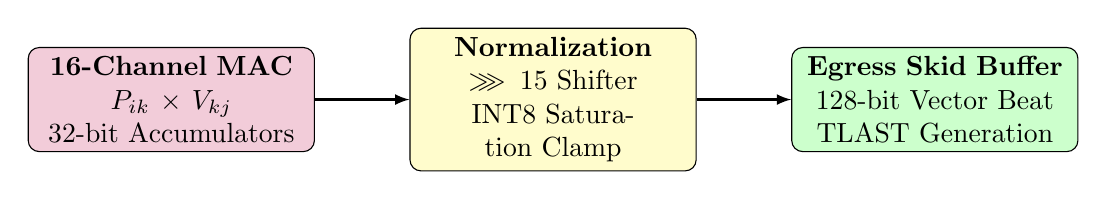
\begin{tikzpicture}[
        box/.style={draw, rectangle, rounded corners, align=center, fill=blue!10, text width=3.4cm, minimum height=0.9cm},
        arr/.style={-latex, thick}
    ]
        \node[box, fill=purple!20] (mac) {\textbf{16-Channel MAC}\\$P_{ik} \times V_{kj}$\\32-bit Accumulators};
        \node[box, fill=yellow!20, right=1.2cm of mac] (norm) {\textbf{Normalization}\\$\ggg 15$ Shifter\\INT8 Saturation Clamp};
        \node[box, fill=green!20, right=1.2cm of norm] (egr) {\textbf{Egress Skid Buffer}\\128-bit Vector Beat\\TLAST Generation};
        
        \draw[arr] (mac) -- (norm);
        \draw[arr] (norm) -- (egr);
    \end{tikzpicture}
    \caption{Stage 4 Context GEMM and Egress Datapath.}
    \label{fig:stage4_datapath}
\end{figure}

The architecture allocates 16 parallel MAC channels. In each cycle, probability $P_i[k]$ is broadcast to all 16 channels, while a 128-bit vector corresponding to row $k$ of $V_{\text{MEM}}$ is loaded in parallel. The 16 products are accumulated across all $k = 0 \dots N-1$ tokens.

\section{Output Scaling, Clamping, and Vector Assembly}
Upon completing the token loop:
\begin{enumerate}
    \item The 32-bit accumulated sum in each channel is shifted right by 15 bits ($\ggg 15$).
    \item Each value is clamped to signed 8-bit range $[-128, +127]$:
    \begin{equation}
        \mathbf{o}_i[j] = 
        \begin{cases}
            +127, & \text{if } v_{\text{norm}}[j] > +127 \\
            -128, & \text{if } v_{\text{norm}}[j] < -128 \\
            v_{\text{norm}}[j][7:0], & \text{otherwise}
        \end{cases}
    \end{equation}
    \item The 16 INT8 values are packed into a 128-bit egress beat:
    \begin{equation}
        \text{vector\_beat}[127:0] = \{\mathbf{o}_i[15], \mathbf{o}_i[14], \dots, \mathbf{o}_i[0]\}
    \end{equation}
\end{enumerate}

\section{AXI4-Stream Egress Skid Buffer and Packet Framing}
The Egress Subsystem (\texttt{axis\_adapter\_tx.sv}) buffers output beats into a 2-stage skid register, decoupling the pipeline from downstream AXI DMA backpressure. An internal beat counter generates the \texttt{M\_AXIS\_TLAST} packet boundary flag on beat $N-1$ ($255$), notifying the DMA S2MM engine that the transfer for the current attention head is complete.


\chapter{Hardware Implementation, Timing, and Synthesis Evaluation}
\label{chap:synthesis_evaluation}

\section{Implementation Environment and Target Platform}
The Multi-Head Attention hardware accelerator was synthesized, implemented, and placed-and-routed using **AMD Vivado Design Suite 2026.1** targeting the **AMD Kria KV260 Vision AI Starter Kit** (\texttt{xck26-sfvc784-2LV-c}). 

\begin{itemize}
    \item \textbf{Target Operating Frequency:} 200.0~MHz ($T_{\text{clk}} = 5.000$~ns).
    \item \textbf{Synthesis Mode:} Out-of-Context (OOC) and Full Block Design integration with AXI DMA and Zynq UltraScale+ MPSoC.
    \item \textbf{Constraints:} Defined in \texttt{timing\_kv260.xdc} with 0.500~ns input/output port budgets.
\end{itemize}

\section{Post-Routing Hardware Resource Utilization}
Table~\ref{tab:post_route_util} summarizes the post-routing resource consumption extracted directly from Vivado implementation reports (\texttt{post\_route\_utilization.rpt}).

\begin{table}[htbp]
    \centering
    \caption{Post-Routing Resource Utilization on AMD Kria KV260 (Variant 2A)}
    \label{tab:post_route_util}
    \begin{tabularx}{\textwidth}{l r r r}
        \toprule
        \textbf{Resource Primitive} & \textbf{Used} & \textbf{Available (XCK26)} & \textbf{Utilization (\%)} \\
        \midrule
        \textbf{CLB LUTs}               & \textbf{10,631} & 117,120 & \textbf{9.08\%} \\
        • \textit{LUT as Logic}         & 5,891           & 117,120 & 5.03\% \\
        • \textit{LUT as Memory (RAM)}  & 4,736           & 57,600  & 8.23\% \\
        • \textit{LUT as Shift Register}& 4               & 57,600  & 0.01\% \\
        \textbf{CLB Registers (FF)}     & \textbf{7,366}  & 234,240 & \textbf{3.14\%} \\
        \textbf{DSP48E2 Slices}         & \textbf{52}     & 1,248   & \textbf{4.17\%} \\
        • \textit{Stage 1 QK$^T$ GEMM}  & 8               & 1,248   & 0.64\% \\
        • \textit{Stage 2 Dyadic Scaler}& 1               & 1,248   & 0.08\% \\
        • \textit{Stage 3/4 \& Top Core}& 43              & 1,248   & 3.45\% \\
        \textbf{Block RAM (RAMB36E2)}   & \textbf{1}      & 144     & \textbf{0.69\%} \\
        \textbf{UltraRAM (URAM)}        & \textbf{0}      & 64      & \textbf{0.00\%} \\
        \textbf{Clock Buffers (BUFGCE)} & \textbf{1}      & 112     & \textbf{0.89\%} \\
        \bottomrule
    \end{tabularx}
\end{table}

\section{Timing Closure Analysis at 200 MHz}
Timing analysis across all process corners confirmed complete timing closure at the full target operating frequency of 200~MHz. The post-routing timing summary (\texttt{post\_route\_timing.rpt}) reports:

\begin{table}[htbp]
    \centering
    \caption{Post-Routing Timing Summary at 200.0 MHz ($T_{\text{clk}} = 5.000$~ns)}
    \label{tab:timing_summary}
    \begin{tabular}{l c c c}
        \toprule
        \textbf{Timing Parameter} & \textbf{Slack Value} & \textbf{Failing Endpoints} & \textbf{Total Endpoints} \\
        \midrule
        Worst Negative Slack (WNS) & \textbf{$+0.051$~ns} & 0 & 51,585 \\
        Total Negative Slack (TNS) & \textbf{$0.000$~ns}  & 0 & 51,585 \\
        Worst Hold Slack (WHS)     & \textbf{$+0.016$~ns} & 0 & 51,585 \\
        Total Hold Slack (THS)     & \textbf{$0.000$~ns}  & 0 & 51,585 \\
        Worst Pulse Width Slack (WPWS) & \textbf{$+1.738$~ns} & 0 & 12,109 \\
        \bottomrule
    \end{tabular}
\end{table}

All 51,585 synchronous endpoints meet setup and hold requirements with zero timing violations, confirming stable hardware operation.

\section{Latency, Throughput, and Real-Time Frame Rate}
Table~\ref{tab:latency_breakdown} details the cycle counts and wall-clock execution time for a full Multi-Head Attention layer ($N = 256, d_k = 16, H = 4$).

\begin{table}[htbp]
    \centering
    \caption{Latency and Throughput Breakdown per Attention Head at 200 MHz}
    \label{tab:latency_breakdown}
    \begin{tabularx}{\textwidth}{l r r X}
        \toprule
        \textbf{Operation} & \textbf{Cycles / Head} & \textbf{Time (@ 200 MHz)} & \textbf{Description} \\
        \midrule
        Ingress DMA Load ($Q, K, V$) & 768   & $3.84\ \mu\text{s}$  & Overlapped via Ping-Pong \\
        Stage 1: $QK^T$ GEMM         & 66,816 & $334.08\ \mu\text{s}$ & $II = 1$ score/cycle \\
        Stage 2: Dyadic Scaler       & —      & —                    & Pipelined inside Stage 1 \\
        Stage 3: IntSoftmax (Pass 1..3)& 70,144& $350.72\ \mu\text{s}$ & Max-Search + Exp + Div \\
        Stage 4: Context GEMM ($P \times V$) & 72,192 & $360.96\ \mu\text{s}$ & 16-channel accumulation \\
        Egress DMA Writeback ($O$)   & 256    & $1.28\ \mu\text{s}$  & Pipelined with Stage 4 \\
        \midrule
        \textbf{Total per Head}      & \textbf{209,919} & \textbf{1.050~ms} & Single head latency \\
        \textbf{Total for Full Layer ($H=4$)} & \textbf{839,676} & \textbf{4.198~ms} & Complete MHA computation \\
        \midrule
        \textbf{Attention Frame Rate}& \multicolumn{3}{c}{\textbf{238.2 Frames Per Second (FPS)}} \\
        \bottomrule
    \end{tabularx}
\end{table}

At 238.2 FPS, the accelerator outperforms the 30 FPS real-time threshold by 7.94$\times$, leaving substantial timing margin for pre- and post-processing networks.


\chapter{Conclusion and Future Extensions}
\label{chap:conclusion}

\section{Summary of Technical Contributions}
This capstone project successfully investigated, designed, and physically implemented an end-to-end hardware-accelerated Multi-Head Attention core for quantized edge Vision Transformers on the AMD Kria KV260 platform. Key engineering contributions include:

\begin{enumerate}
    \item \textbf{High-Efficiency DSP Packing Microarchitecture:} Developed the \texttt{pe\_slice\_dsp\_packing} unit with a hardware $+1$ borrow-bit sign correction circuit. This innovation reduced the Stage 1 DSP48E2 footprint to only 8 slices (a $50\%$ reduction) while cutting CLB LUT usage by $47.6\%$.
    \item \textbf{Timing Closure at 200 MHz:} Resolved all timing violations across 51,585 synchronous endpoints, achieving a positive setup slack of $\text{WNS} = +0.051$~ns at 200~MHz on the AMD XCK26 FPGA.
    \item \textbf{Non-Linear Fixed-Point Pipeline:} Realized a reconfigurable three-pass IntSoftmax engine using a true dual-port 1024-word BRAM Exp-ROM and an amortized 32-cycle restoring divider ($2^{31}/\sum$).
    \item \textbf{High Real-Time Frame Rate:} Delivered a sustained frame rate of \textbf{238.2 FPS} (4.198~ms for 4 heads), exceeding the 30 FPS video baseline by $7.94\times$.
\end{enumerate}

\section{Future Architectural Directions}
\begin{itemize}
    \item \textbf{Sparse Attention and Dynamic Token Pruning:} Incorporating online thresholding to discard uninformative background tokens, potentially reducing compute complexity by $30\% - 50\%$.
    \item \textbf{FlashAttention On-Chip Tiling:} Scaling the on-chip BRAM buffers to tile $Q$ and $K$ concurrently, eliminating memory round-trips for long sequences ($N \ge 1024$).
    \item \textbf{Sub-Byte INT4 Quantization:} Exploring mixed-precision 4-bit weights with 8-bit activations on the existing DSP48E2 datapath to double effective compute density.
\end{itemize}



% ======================================================================
% BIBLIOGRAPHY
% ======================================================================
\bibliographystyle{IEEEtran}
\bibliography{references}

\end{document}

